\documentclass[12pt, a4paper]{article}
\author{Aaron Berger\qquad Christopher Chute\qquad Matthew Stone}
\title{Query Complexity of Mastermind Variants}
\usepackage[bottom=1.2in, left=0.75in, right=0.75in, top=1in]{geometry}
\usepackage{amsmath, amsthm, amssymb}
\newtheorem{lem}{Lemma}
\usepackage{graphicx}
\usepackage{setspace}
\usepackage{enumitem}
\usepackage{booktabs}
\usepackage{footnote}
\usepackage[english]{babel}
\usepackage[utf8]{inputenc}
\usepackage[nottoc]{tocbibind}

% 	 \begin{header footer formatting}
%    \usepackage{fancyhdr}
%    \setlength{\headheight}{48pt}
%    \pagestyle{fancyplain}
%    \lhead{Mastermind Project: \textit{Notes}\\\today{}}
%    \rhead{AB, CC, MS}
%    \rfoot{\thepage}
%    \cfoot{}
% 	 \end{header footer formatting}

% remove ``*'' for numbered theorems
\newtheorem{theorem}{Theorem}
\newtheorem{lemma}{Lemma}

% \begin{pretty i-hat and j-hat}
\newcommand*{\ihat}{\hat{\imath}}
\newcommand*{\jhat}{\hat{\jmath}}
\newcommand*{\jwidehat}{\widehat{\jmath}}
% \end{pretty i-hat and j-hat}

% ********************************* END OF PREAMBLE ***********************************

\begin{document}
\maketitle

\begin{abstract}
We analyze variants of the popular board game Mastermind. In this two-player game,
the codebreaker submits queries with the goal of identifying a hidden
sequence, constructed at the beginning of the game by the codemaker. At each step,
the codebreaker receives feedback in the form of ``black'' and ``white'' hits
and incorporates the response into his next guess. We discuss asymptotics for the
number of guesses needed to identify an unknown $n$-vector constructed from $k$
possible colors. We look at strategies that receive two-color responses, as well as
black hit-only responses. We consider both allowing and prohibiting repeated
colors in the hidden sequence, and we analyze both adaptive and non-adaptive guessing
strategies.
\end{abstract}

\section{Introduction}
Mastermind is a two-player board game that was invented in 1970, and variants on its
basic four-spot, six-color structure have been studied extensively.
In the original game, there are two players: the codemaker and the codebreaker.
The codemaker initiates a game by constructing a 4-vector $p$ from the six available
colors, and the codebreaker attempts to guess the hidden vector in as few turns as
possible. A turn consists of two parts: First the codebreaker submits a query vector
$q$, which has the same form as a hidden vector. Second, the codemaker gives a
two-part response:
	\begin{enumerate}[label=\arabic*.]
	\item Black Hits: The number of correct colors in the correct spot
	(the number of positions $i$ such that $q_i=p_i$).
	\item White Hits: The number of correct colors in the incorrect spot, and which
	have not been used in another hit.
	\end{enumerate}
In 1976, Donald Knuth presented a greedy ``minimax'' algorithm, and he showed via
computer simulation that his algorithm always guesses the hidden vector in five turns
or fewer \cite{DK76}. Moreover, the minimax algorithm for Mastermind is optimal in
the worst case---there is no algorithm that can guarantee to win in at most four turns.
\footnote{Knuth shows that the worst-case response to any possible first guess leaves
at least 256 possible solution vectors. After this, with 14 possible responses per turn,
the trivial information-theoretic argument gives a lower bound of five turns total to win.}

There are multiple natural extensions to the original Mastermind game. Varying the
number of spots $n$ and colors $k$, as well as the relationship between $n$ and $k$,
is one such extension. In this paper, we also consider both allowing and prohibiting
repeated colors in vectors, and we examine both dual-color and black-only responses.
We explore another degree of freedom between adaptive strategies, in which the
codebreaker receives responses and adjusts the next guess accordingly, and non-adaptive
strategies, in which all guesses are submitted at the beginning of the
game and the hidden vector must be uniquely determined by the sequence of responses.
\footnote{Note that in a non-adaptive guessing strategy, our guesses need to
\textit{identify} the hidden vector rather than guess it outright. That is, a
non-adaptive strategy wins if the sequence of responses to the guess vectors allows
the codebreaker to distinguish between all possible hidden vectors. It is not
necessary that a winning set of non-adaptive guesses includes the hidden vector
itself.}

\subsection{Previous Work}
Original analysis of the game was performed by Knuth, who laid out the minimax algorithm. \cite{VC83}, and later \cite{DS13}, were able to successfully resolve the adaptive and non-adaptive games with repeated colors variant when there are fewer colors than spots. They also describe algorithms for the standard game for more colors than spots. \cite{KT86}, and later \cite{OS13}, provide algorithms for the no-repeats variant of the game. 

\subsection{Our Contribution}
We primarily focus on three new methods for worst-case analysis of mastermind games where the number of colors
$k$ is greater than or equal to the number of spots $n$. Unlike the case where $k < n$,
there are barely any tight bounds for any variant of the game, and some commonly analyzed
variants have no upper bounds at all. We first show an upper bound of $nk$ for any mastermind
game. We perform the first ever worst-case analysis of Knuth's minimax algorithm and show
that it eliminates at least a fraction of $1/nk$ of the remaining solutions at any step, for an 
$O(n^2k \log k)$ upper bound. Additionally, we perform analysis on a new lower bound that
models a set of best guesses such that the distribution of the responses among the solutions
approaches an even distribution (the best possible distribution) as quickly as possible. With this
analysis, we obtain an improvement over the trivial lower bound (on the permutation game) with a new bound of $n- \log \log n$ turns.
Next, we extend two arguments by \cite{DS13}: one for the black-peg NO-REPEATS game to 
give an $n \log k$ lower bound, and one to the original non-adaptive game for an $O(k \log k)$ 
upper bound. Finally, we end with a few notes and conjectures about the different variants of
the game when the number of colors far exceeds the number of spots.
\section{Standard Upper Bound}
The standard upper bound of $nk$ turns for any game is derived as follows: \\
For a game of mastermind with $n$ spots and $k$ colors (with or without repeats), every
hidden vector and query can be represented by a matrix $A\in\mathbb{R}^{n\times k}$,
defined by $A_{ij}=1$ if the $i$-th peg is the $j$-th color, and 0 otherwise.
In that way, for a given hidden vector matrix $X$ and query matrix $Q$,
the codemaker's black-peg response to the query is given by $X\cdot Q$.
(We are treating these matrices as vectors in $\mathbb R^{nk}$.)
Let $S$ be the subspace spanned by the set of possible queries. 
Then there must exist a basis of queries,
$K$, with $|K|=\text{dim}(S)$ and $K$ spanning $S$. $S\subset \mathbb{R}^{n\times k}$,
so $\text{dim}(S)\le \text{dim}(\mathbb{R}^{n\times k})=n\cdot k$.
Now, we choose this basis as our set of guesses. We look at the black-hit responses to 
these guesses, which gives us the dot-products of the hidden vector $X$ with each of
the basis vectors. By distribution, we can then uniquely determine the dot-products of 
$X$ with each of the basis vectors of some arbitrary orthogonal basis of $S$, and we can
then determine the projections of $X$ onto each basis vector in this orthogonal basis.
Adding these components together allows us to uniquely determine $X \in S$. 
Thus, there exists a set of at most $n\cdot k$ queries which uniquely determines every
possible hidden permutation. (Note that since this strategy is non-adaptive and only
uses black hits, this bound holds for every variant of the game analyzed in this paper.)
\section{Adaptive Strategies}
We begin by performing an analysis on the PERMUTATION game, which is the NO-REPEATS
game where the number of spots $n$ equals the number of colors $k$. Algorithms for this game
that take $O(n \log n)$ turns were developed by \cite{KT86} and \cite{OS13}. The
information-theoretic lower bound on this game is $n - n/ \log n + O(1)$. We improve this to 
$n - \log n$ for small $n$, and $n- \log \log n$ for sufficiently large $n$, which constitutes, 
to our knowledge, the first improvement over the trivial information-theoretic lower bound
for any adaptive mastermind game. \\
\subsection{Lower Bound on the Permutation Game}
\begin{enumerate}
\item \textit{Trivial Lower Bound.}
	We have $n!$ possible hidden vectors, and each query has $n$ possible
	responses.\footnote{The possible responses are $0, 1, \ldots, n-2,$ and $n$, since it is
	impossible to get exactly $n-1$ black hits with no repeats and $n=k$.}
	Since we must distinguish between every pair of vectors, we must ask at least
		\begin{equation*}
		\log_{n}(n!) = n-\frac{n}{\ln(n)}+O(1)
		\end{equation*}
	
	\item\textit{Buckets.}
	In order to beat the trivial lower bound, we use a more accurate picture
	of the distribution of the possible solutions after feedback from a given guess.
	For any guess, we can split the possible solutions up into groups, which
	we will call \textit{buckets}; one bucket for each possible response given by
	the codemaker. For any guess we make, the number of possible solutions that give
	the response ``$k$ (black) hits'' is the number of permutations with $k$ fixed
	points with respect to our guess vector.
	\begin{center}
	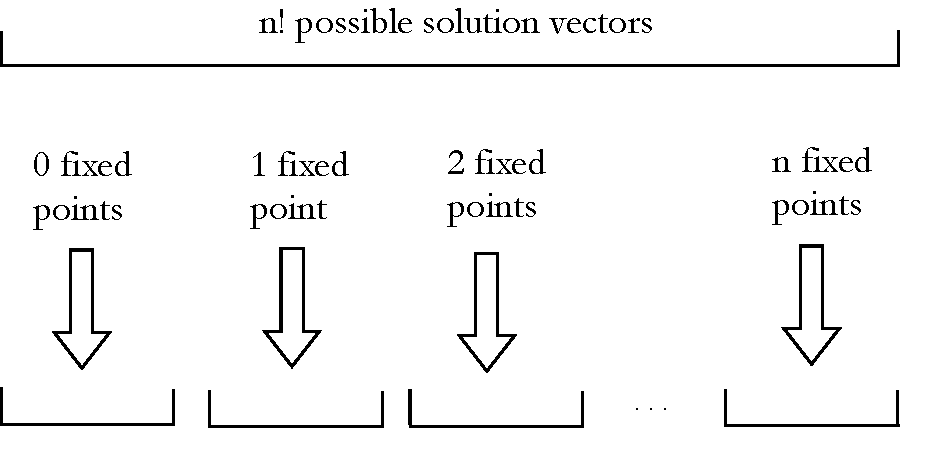
\includegraphics[keepaspectratio=true, width=0.7\textwidth]{buckets.pdf}
	\end{center}
	The size of a bucket of possible
	solutions with $k$ hits can be counted easily: we choose the $k$ colors that are
	fixed points (with respect to our guess vector), then we permute the remaining $n-k$ colors
	without any fixed points, giving $D(n - k)$, the derangements on an $(n-k)$-element
	vector:
		\begin{equation*}
		\binom{n}{k}D(n-k)
		\end{equation*}
	This tells us the initial size of each bucket (by symmetry, this is the same distribution
	for any guess). In general, the buckets start out large,
	and decrease approximately by a factor of $x$ from the $(x-1)$ bucket to the
	$x$ bucket. It is important to note that if we look at the sizes of these buckets for
	a particular guess
	part-way into the game, the size of each bucket can only decrease from its original size,
	as each previous guess simply eliminates some solutions from each bucket.
	
	\item\textit{Notation.}
	We let $S_{n}(t)$ be a lower bound on the minimum number of possible solutions remaining
	after $t$ guesses for any guessing strategy. We compute this lower bound by using
	a hypothetical set of guesses which are each guaranteed to eliminate at least as 
	many solutions as any other guess we could make at any point in the game. 
	The worst-case scenario for this set of guesses
	therefore provides a lower bound for the number of guesses required by any
	guessing strategy to guarantee finding the hidden vector.
	
	\item\textbf{Recurrence Relation on Number of Possible Solutions after $t$ Turns:}
		\begin{enumerate}
		\item We will inductively prove a lower bound, $S_{n}(t)$. By the
		discussion above,
		we know the maximum possible size of each bucket.
		The best possible guess distributes the remaining solutions as evenly as
		possible so that the bucket containing the most remaining solutions is as
		small as possible. This best-possible distribution will fill some number of
		smaller buckets entirely and split the remaining solutions evenly
		into some number $x$ larger buckets. That is, there are $x$ incompletely
		filled buckets.
		
		\item At the beginning of the $t$-th turn, we have at least $S_{n}(t-1)$
		possible
		solutions remaining. As we showed before, the size of each bucket is bounded
		by its original size of $\binom{n}{k}D(n-k)$. Thus the number of solutions
		remaining $(t-1)$-th turn relates to the value of $S_{n}(t)$ as follows:
		
		Let $B_i(t)$ be the exact number of possible solutions remaining in the
		bucket holding possible solutions with $i$ fixed points during the
		$t$-th turn (after submitting the guess vector, but before feedback). So
		\begin{align*}
		S_{n}(t-1) & = \sum_{i = 0}^{n}B_i(t)\\
		& = \sum_{i=0}^{x-1}B_i(t) + \sum_{i=x}^{n}B_i(t)\\
		& \le \sum_{i = 0}^{x-1}S_n(t) + \sum_{i=x}^{n}\binom{n}{i}D(n-i)\quad
		\text{for optimal $x$}\\
		& = x\cdot S_{n}(t) + \sum_{i = x}^{n}\binom{n}{i}D(n-i)
		\end{align*}
		Once we know $S_{n}(t)$, picking $x$ too large results in some smaller boxes
		overfilled. Picking $x$ too small results in some larger boxes overfilled. So
		changing $x$ to be something other than optimal always increases the RHS
		of this equation. Thus we have
		\begin{align*}
		S_{n}(t-1) & \le x\cdot S_{n}(t) + \sum_{i=x}^n\binom{n}{i}D(n-i)\quad\forall x
		\end{align*}
		Where $t$ is the number of turns taken, $S_{n}(t)$ is the number of possible
		solutions remaining after the $t$-th turn, and $D(k)$ is the derangements
		on a set of size $k$.
		\end{enumerate}
		
		\item\textit{Claim.}
			\begin{equation*}
			\sum_{i=x}^n\binom{n}{i}D(n-i) \le \frac{n!}{x!}
			\end{equation*}
			This inequality leads to our bound on $S_{n}(t)$ given
			below.\footnote{A combinatorial argument can be made as follows: The LHS
			denotes the number of permutations of an $n$-element vector which have
			at least $x$ fixed points. Suppose we choose $x$ fixed points and
			simply permute the rest of the vector. This gives $\binom{n}{x}(n-x)!
			=\frac{n!}{x!}$ possible permutations. Clearly this includes all
			vectors with at least $x$ fixed points (and over-counts by some
			margin), so the inequality holds.}
			\begin{proof}
				\begin{align*}
				\sum_{i=x}^n\binom{n}{i}D(n-i) & =
				\frac{n!}{x!}\sum_{i=x}^{n}\frac{x!}{i!(n-i)!}D(n-i)\\
				& \qquad\text{we use the fact that }\frac{x!}{i!}\le\frac{1}{(i-x)!}\\
				& \le \frac{n!}{x!}\sum_{i=x}^{n}\frac{1}{(i-x)!(n-i)!}D(n-i)\\
				& \qquad\text{let $k=i-x$}\\
				& = \frac{n!}{x!}\sum_{k=0}^{n-x}\frac{1}{k!(n-x-k)!}D(n-x-k)\\
				& = \frac{n!}{x!(n-x)!}\sum_{k=0}^{n-x}\binom{n-x}{k}D(n-x-k)\\
				& \qquad\text{note the summation counts all possible permutations}\\
				& = \frac{n!}{x!(n-x)!}(n-x)!\\
				& = \frac{n!}{x!}				
				\end{align*}
			\end{proof}		
		\begin{enumerate}
		\item Plug the above result into the inequality to get
			\begin{equation*}
			S_{n}(t-1) \le x\cdot S_{n}(t) + \frac{n!}{x!}
			\end{equation*}
		So we have
			\begin{equation*}
			S_{n}(t)\ge \frac{1}{x}\left(S_{n}(t-1)-\frac{n!}{x!}\right)
			\end{equation*}
		\end{enumerate}
	\end{enumerate}
		\begin{lemma} For all $n$, and for any constant $C_n$, we have
			\begin{equation*}
			\frac{S_{n}(t)}{n!}\ge \frac{C_{n}! - (H_{C_{n}+t} - H_{C_{n}})}{(C_n+t)!}
			\end{equation*}
			\begin{equation*}
			\text{where }\quad0\le t\le n-C_{n}
			\end{equation*}
		\end{lemma}
	Here we use $H_n$ to denote the $n$-th harmonic number.\footnote{$H_n=\sum_{i = 1}
	^n\frac{1}{i}$}
		\begin{proof}
		While this equation holds for all $x$, to achieve a desirable bound, we will
		let $x=t+C_{n}$ for any positive constant $C_{n}$. We have
		\begin{enumerate}[label=]
		\item\textit{Base Case.} When $t=0$, we have $S_n(0)= n!$ and
			\begin{equation*}
			\frac{S_{n}(0)}{n!}\ge \frac{C_{n}! - (H_{C_{n}}-H_{C_{n}})}{C_{n}!} = 1
			\end{equation*}
			
		\item \textit{Inductive Step.} Assume the induction hypothesis holds for $t-1$.
			\begin{align*}
			\frac{S_{n}(t)}{n!}
			& \ge \frac{1}{x}\left(\frac{S_{n}(t-1)}{n!}-\frac{1}{x!}\right)
			\end{align*}
		Let $x=C_{n}+t$.
			\begin{align*}
			\frac{S_{n}(t)}{n!}
			& \ge \frac{1}{C_{n}+t}\left(\frac{S_{n}(t-1)}{n!}
			-\frac{1}{(C_{n}+t)!}\right)
			\end{align*}
		Inductively,
			\begin{align*}
			\frac{S_{n}(t)}{n!}
			& \ge \frac{1}{C_{n}+t}\left(\frac{C_{n}!-(H_{C_{n}+t} - H_{C_{n}})}
			{(C_{n}+t-1)!} - \frac{1}{(C_{n}+t)!}\right)\\
			& \ge \left(\frac{C_{n}! - (H_{C_{n}+t-1} - H_{C_{n}}) - \frac{1}{C_{n}+t}}
			{(C_{n}+t)!}\right)\\
			& \ge \left(\frac{C_{n}! - (H_{C_{n}+t} - H_{C_{n}})}{(C_{n}+t)!}\right)
			\end{align*}
			Then
			\begin{align*}
			S_{n}(n-C_{n}) & \ge n!\left(\frac{C_{n}! - (H_n - H_{C_{n}})}{n!}\right)\\
			& \ge C_{n}! - (H_n-H_{C_{n}})
			\end{align*}
		Thus the inequality holds for all $n$.
		\end{enumerate}
		\end{proof}
		We choose $C_{n}$ by the following reasoning: we want to achieve a lower bound
		of $n-C_{n}$ turns. Thus, we want $S_n(n-C_{n})>1$, which follows if
		\begin{equation*}
		C_{n}! - (H_n - H_{C_{n}}) > 1
		\end{equation*}
		For $C_{n}=\log\log n$, this is $\ge 1$ for $n\ge e^{198}$.\\
		For $C_{n}=\log n$, this is true for $n\ge 10$.
		
 	In conclusion, when $n$ is sufficiently large, the minimum number of remaining
	possible solutions after $n - \log\log n$ guesses is at least
		\begin{align*}
		S_n(n-\log\log n) & \ge (\log\log n)! - (H_n - H_{\log\log n})\\
		& > 1
		\end{align*}
	Thus there is no strategy that can reduce the set of possible solutions to
	one, and guarantee finding the codemaker's hidden vector, in $n-\log\log n$
	turns or fewer.
\subsection{Best Guesses and the Minimax Algorithm}
We now move on to an analysis of the best possible guesses and the minimax algorithm. Here, 
the best possible guess is defined in the same way as \cite{DK76}: it is the one such that the 
maximum number of solutions remaining over all responses is minimized (equivalently, the 
minimum number of solutions eliminated over all responses is maximized). This is the guess
chosen by the minimax algorithm. \\
We begin by analyzing the NO-REPEATS game.

\begin{theorem} In Mastermind with no repeats with $n$ spots and $k$ colors,
	for any set of possible remaining solutions, there exists a
	guess vector for which any response will eliminate at least $1/nk$ of the
	remaining solutions.
	\end{theorem}
	\begin{enumerate}
	\item\textit{Notation.}
		\begin{enumerate}[label=\roman*.]
		\item\textit{Basics.} Let $n$ be the number of spots in the hidden vector.
		Let $k$ be the number of colors available. Since we allow no repeats in this
		variant of Mastermind, we have $k\ge n$. We will use single-count responses,
		which are the number of spots in which our guess vector and the hidden vector
		have the same color in that spot.
		\item\textit{Remaining Solution Set.} As the game proceeds, we maintain a set
		$S$ that contains all possible solution vectors that haven't been ruled out
		by a previous guess and response.
		\item\textit{Bucket.} As defined in the previous section, a guess splits
		the remaining possible solutions into ``buckets,'' where a bucket $B_i$
		contains all the remaining possible solutions with $i$ fixed points with
		respect to the guess vector.
		\item\textit{Sub-Bucket.} Within a bucket, we will divide the vectors
		based on a chosen component, say the first element of each vector.
		Then there will be $k$ sub-buckets $D_i$, where $D_1$ contains all vectors
		from the bucket with a $1$ in the first spot, $D_2$ contains all those
		with a $2$ in the first spot, and so on.
		\end{enumerate}

	\item
		\begin{proof}
		We give a proof by induction on $n$.
			\begin{enumerate}[label=]
			\item\textit{Base Case.} When $n=1$, we have a single-element vector.
			So there are at most $k$ possible solutions remaining at any step, thus
			$|S|\le k$. If we guess one of the remaining solutions $v\in S$, this
			will eliminate $1$ solution ($v$ itself) if the response is $0$
			and $|S|-1$ solutions if the response is $1$. So we're guaranteed to
			eliminate at least $1/|S|\ge 1/(nk)$ solutions.
			
			\item\textit{Inductive Step.} Assume that for $n-1$ spots and any number
			of colors $\widehat{k}$ (where $n\ge 2$), we are guaranteed that
			there is a guess that eliminates a fraction at least $1/(n\widehat{k})$
			of the solutions.
			
			Consider a guess vector $\sigma=\{\sigma_1, \sigma_2, \ldots, \sigma_n\}$.
			We will analyze the number of solutions
			eliminated from $S$ by guessing $\sigma$ in the worst-case. We divide $S$
			into $n$ buckets $B_1, B_2, \ldots, B_n$, where $B_i$ is as defined above
			($i$ fixed points with respect to $\sigma$). Consider the response $j$
			that eliminates as few possible solutions as possible from $S$,
			so $|B_j| = \max\{|B_1|, |B_2|, \ldots, |B_n|\}$.
			
			Suppose that
				\begin{equation*}
				|B_j|\le\frac{nk - 1}{nk}\cdot|S|
				\end{equation*}
			Then the response $j$ would eliminate at least $|S|/(nk)$ solutions from
			$S$, and since $j$ eliminates the fewest possible solutions of any
			response, all responses to $\sigma$ eliminate a fraction at least
			$1/(nk)$ of the possible solutions in $S$.
			
			Otherwise we have
				\begin{equation*}
				|B_j|>\frac{nk - 1}{nk}\cdot|S|
				\end{equation*}
			\textit{Case 1.} If $j>0$, the total number of hits among all vectors in
			$B_j$ is $j\cdot |B_j|$. These hits are divided up among $n$ spots,
			therefore by the pigeonhole principle, at least one position
			must have at least
				\begin{align*}
				\frac{j}{n}\cdot|B_j|
				\end{align*}
			Vectors that match the guess at that spot. WLOG, we assume this is
			position one. We now divide the bucket $B_j$ into sub-buckets $D_i$,
			where permutation $s\in B_j$ is put into sub-bucket $D_{s_1}$. From above,
			we have 
			\begin{equation*}
			|D_{\sigma_1}|\ge \frac{j}{n}\cdot|B_j|
			\end{equation*}
			We have two sub-cases:
				\begin{enumerate}[label=\roman*.]
				\item $|D_{\sigma_1}|\le \dfrac{n-1}{n}\cdot|B_j|$:\\
				Then we apply the pigeonhole principle on the remaining solutions
				in $B_j$ to find the second-largest sub-bucket:
				By our assumption, there are at least $|B_j|/n$ solutions remaining
				in $B_j$, and there are $k-1$ remaining sub-buckets $D_i$. By the
				pigeonhole principle, there exists a $D_\alpha$ such that 
				\begin{equation*}
				|D_\alpha| \ge \frac{1}{n}\cdot\frac{1}{k-1}\cdot|B_j|
				\end{equation*}
				If $\alpha$ is an element of $\sigma$, then WLOG
    			let the color be $\sigma_2$. Then in this case we consider the
				guess vector
    			$\overline{\sigma}=\{\sigma_2, \sigma_1, \sigma_3, \ldots, \sigma_n\}$.
    			Otherwise, consider the guess vector
    			$\overline{\sigma}=\{\alpha, \sigma_2, \sigma_3, \ldots, \sigma_n\}$.
				Consider the buckets $C_i$ formed from the guess vector
				$\overline{\sigma}$. In either case, the vectors in $D_{\sigma_1}$ will
				have at least one fewer hit with $\overline{\sigma}$ than with
				$\sigma$, and the guess vectors in $D_{\alpha}$ will have at least
				one more hit. Therefore, any response to $\overline{\sigma}$ which
				corresponds to some vectors in $D_{\sigma_1}$ corresponds to none
				of the vectors in $D_{\alpha}$ and vice versa. So we know that any
				response to $\overline{\sigma}$ will entirely eliminate at least one
				of those two sets. From above, we know
					\begin{align*}
					|D_{\sigma_1}| & \ge \frac{j}{n}\cdot|B_j|\\
					& \ge \frac{j}{n}\cdot\frac{nk-1}{nk}\cdot|S|\\
					& \ge \frac{1}{n}\cdot\frac{n}{nk}\cdot|S|\\
					& = \frac{1}{nk}\cdot|S|
					\end{align*}
				And
					\begin{align*}
					|D_\alpha| & \ge\frac{1}{n}\cdot\frac{1}{k-1}\cdot|B_j|\\
					& \ge \frac{1}{nk-n}\cdot\frac{nk-1}{nk}\cdot|S|\\
					& \ge \frac{1}{nk}\cdot|S|
					\end{align*}
				Since $\overline{\sigma}$ will always eliminate at least one of
				these two sets, we also have that $\overline{\sigma}$ will eliminate
				at least $|S|/(nk)$ vectors from $S$ with any response.
					
				\item $|D_{\sigma_1}|> \dfrac{n-1}{n}\cdot|B_j|$:\\
				Consider the set of vectors in $D_{\sigma_1}$. By definition,
				all of them have $\sigma_1$ as their first entry. Their remaining
				$n-1$ entries are made up of the remaining $k-1$ colors, and no two of
				them coincide in all spots $2, 3, \ldots, n$ (otherwise they would be
				the same vector). Therefore, if we consider this new set of $n-1$
				vectors formed by taking spots $2, 3, \ldots, n$ of each vector in
				$D_{\sigma_1}$, they are a set of possible solutions for this
				Mastermind game with $n-1$ spots and $k-1$ colors. By the induction
				hypothesis, there is a guess of size $n-1$ that is guaranteed to
				eliminate $1/((n-1)(k-1))$ of these vectors. If we add $\sigma_1$
				to the
				beginning of this guess, it becomes a guess of size $n$. For any
				response $r$, any of the vectors in $D_{\sigma_1}$ will be eliminated
				if and only if their vector of spots $2, 3, \ldots, n$ was eliminated
				by the response $r-1$ in the smaller game of Mastermind. Therefore,
				this guess still guarantees that we eliminate
				\begin{align*}
				\frac{1}{(n-1)(k-1)}|D_{\sigma_1}|
				& \ge \frac{1}{(n-1)(k-1)}\cdot\frac{n-1}{n}\cdot|B_j|\\
				& \ge \frac{1}{(k-1)}\cdot\frac{1}{n}
				\cdot\frac{nk-1}{nk}\cdot|S|\\
				& \ge \frac{1}{nk-n}\cdot\frac{nk-1}{nk}\cdot|S|\\
				& \ge \frac{1}{nk}\cdot|S|
				\end{align*}
				\end{enumerate}
			
			\textit{Case 2.} If $j=0$, we consider the first component of all vectors
			in the bucket $B_0$. Since $j=0$ and $\sigma=\{\sigma_1, \sigma_2, \ldots,
			\sigma_n\}$, no vector in $B_0$ can contain $\sigma_1$ in the first
			position, so there are $k-1$ possible colors in the first position. By
			the pigeonhole principle, there must be one color which appears in the
			first spot of at least
				\begin{equation*}
				\frac{1}{k-1}\cdot|B_0|
				\end{equation*}
			vectors in $B_0$. If this color appears in $\sigma$, WLOG
			let the color be $\sigma_2$. Then in this case we consider the guess vector
			$\overline{\sigma}=\{\sigma_2, \sigma_1, \sigma_3, \ldots, \sigma_n\}$.
			Otherwise, call this new color $\tau$ and consider the guess vector
			$\overline{\sigma}=\{\tau, \sigma_2, \sigma_3, \ldots, \sigma_n\}$.
			In either case, $\overline{\sigma}$ matches these $|B_0|/(k-1)$ vectors
			in either one or two positions. Consider the
			buckets $C_i$ formed by the guess $\overline{\sigma}$. We know
				\begin{align*}
				|C_1|+|C_2| & \ge \frac{1}{k-1}\cdot |B_0|\\
				& \ge \frac{1}{k-1}\cdot\frac{nk-1}{nk}\cdot|S|\\
				& \ge \frac{1}{k-1}\cdot\frac{nk-n}{nk}\cdot|S|\\
				& = \frac{n}{nk}\cdot|S|\\
				& \ge \frac{2}{nk}\cdot|S|
				\end{align*}
			Therefore we have either
				\begin{equation*}
				|C_1|\ge\frac{1}{nk}\cdot|S|\qquad\text{or}
				\qquad|C_2|\ge\frac{1}{nk}\cdot|S|
				\end{equation*}
			Let this larger bucket be $C_{\alpha}$, then suppose
			\begin{equation*}|C_{\alpha}|\le\frac{nk-1}{nk}|S|\end{equation*}
			Then getting the response $\alpha$ will eliminate at least $|S|/(nk)$
			possible solutions from $S$, and getting any other response will
			eliminate at least $|C_\alpha|\ge |S|/(nk)$ possible solutions. Therefore
			the guess $\overline{\sigma}$ is guaranteed to eliminate at least
			$|S|/(nk)$ solutions from $S$.
			
			Otherwise we have
			\begin{equation*}|C_{\alpha}|>\frac{nk-1}{nk}|S|\end{equation*}
			Then, this satisfies the conditions for Case 1 above, where we have a
			guess whose largest bucket is $B_j$ with $j>0$.
			\end{enumerate}
		\end{proof}
	\item The minimax algorithm is a guessing strategy described by Knuth \cite{DK76}.
	At each turn, the algorithm assigns each of the possible guesses a score equal
	to the minimum number of solutions that they would eliminate over all
	possible responses from the codemaker. It then picks the guess with the maximum
	score.\\\\
	\textit{Corollary.} The minimax algorithm on Mastermind with $n$ spots, $k$
	colors, and no repeats takes at most
		\begin{equation*}
		\frac{\log\left(\frac{k!}{(k-n)!}\right)}{\log\left(\frac{nk}{nk-1}\right)}
		\end{equation*}
	turns to find the hidden vector.
		\begin{proof}
		Each step in the minimax algorithm cuts the set of possible solutions $S$ down
		by a factor of $(nk-1)/(nk)$ at each step. To complete the game, we need to
		cut $S$ down by
			\begin{equation*}
			\frac{1}{\left(\frac{k!}{(k-n)!}\right)}
			\end{equation*}
		Thus the required number of steps is
			\begin{equation*}
			\log_{\left(\frac{nk-1}{nk}\right)}\left(\frac{1}{\frac{k!}{(k-n)!}}\right)
			\end{equation*}
		Which is equivalent to the claim.
		\end{proof}
	This gives us the following asymptotic bounds:
		\begin{enumerate}[label=\roman*.]
		\item The minimax algorithm for Mastermind with $n$ spots, $k$
		colors, and no repeats takes at most $O(n^2k\log k)$ turns to find the
		hidden vector.
		
		\item In the same game where $n=k$, the minimax algorithm takes at most
		$O(n^3\log n)$ turns to find the hidden vector.
		\end{enumerate}
	Both of these asymptotic bounds are actually strict upper bounds, and 
	each of them differs from the exact bound by a constant factor which approaches
	1 as $n$ approaches infinity.
	\end{enumerate}
	
\clearpage
\subsection{Extension of Previous Proof to Repeated Colors}
	In order to replicate the bound of $nk$ with repeated colors, we need to make the
	following assumption:\footnote{The proof in the previous section can be extended
	easily to general $n$ and $k$: Substitute to show that there is always a guess that
	eliminates a factor of $1/n^2k$ possible solutions at each step. For a tighter
	bound with repeated colors, however, we need to make more restrictive assumptions.}
	There exists a guess vector $v$ such that all of the solutions in set $S$
	correspond to a single response $r$ after making the guess $v$. Note that this
	is always satisfied if the solutions are any set of solutions remaining after
	any set of guesses in an actual game of Mastermind. We simply let the guess vector
	$v$ be any guess vector that has already been guessed. Clearly, all solutions
	remaining correspond to whichever response was given to that guess vector, since
	guesses corresponding to any other response were eliminated. We will also prove the
	theorem for the special case of the very first guess separately.
	
	\begin{theorem}
	In a game of Mastermind with $n$ spots and $k$ colors, for any set of remaining
	solutions that can actually be achieved during a game of Mastermind,
	there is always a guess for which any response will eliminate at least
	$1/nk$ of the remaining solutions.
	\end{theorem}
	\begin{proof}
	We will follow the same logic as taken in the previous proof, but will describe
	only the parts that differ from the previous proof.
		\begin{enumerate}
		\item Because of the problem statement, we will separately prove the base
		case where $S$ is the set of all $k^n$ possible solutions before any guesses
		have been made. In this case, we guess the vector $\{1, 1, \ldots, 1\}$. The
		bucket $B_j$ has size
			\begin{equation*}
			|B_j| = \binom{n}{j}(k-1)^{n-j}
			\end{equation*}
		So the greatest fraction of possible solutions remaining is
			\begin{align*}
			\max_{j}\left(\frac{\binom{n}{j}(k-1)^{n-j}}{k^n}\right)
			\end{align*}
		When $k\ge n$, we have
			\begin{align*}
			\frac{\binom{n}{j}(k-1)^j}{k^n}
			& \le \frac{n^{n-j}(k-1)^j}{k^n}\\
			& \le \frac{k^{n-j}(k-1)^j}{k^n}\\
			& = \frac{(k-1)^j}{k^j}\\
			& \le \frac{k-1}{k}
			\end{align*}
		Therefore, we always eliminate a fraction at least $1/k\ge 1/nk$ of the
		solutions.
		
		When $k<n$, it is difficult to find the size of one bucket compared to the
		entire set, so instead we will compare one bucket to the sum of itself
		and the next bucket. This ratio will always be at least the ratio of
		one bucket compared to the entire set.
			\begin{align*}
			\frac{|B_{j+1}|}{|S|}
			& \le \frac{|B_{j+1}|}{|B_j|+|B_{j+1}|}\\
			& \le \frac{1}{\frac{|B_j|}{|B_{j+1}|}+1}\\
			& \le \frac{1}{\frac{\binom{n}{j}(k-1)^{n-j}}
			{\binom{n}{j+1}(k-1)^{n-j-1}}+1}\\
			& \le \frac{1}{\frac{j+1}{n-j}(k-1)+1}\\
			\end{align*}
			We plug in $k \ge 2$ (the entire problem is trivial when $k = 1$, as
			there is only 1 solution).
			\begin{align*}
			\ldots\quad & \le \frac{1}{\frac{j+1}{n-j}+1}\\
			& \le \frac{n-j}{n+1}\\
			& \le \frac{n}{n+1}\\
			& = 1-\frac{1}{n+1}\\
			& \le 1-\frac{1}{nk}
			\end{align*}
		Additionally, for bucket 0, we have:
		\begin{align*}
			\frac{|B_{0}|}{|S|}
			& = \frac{(k-1)^n}{k^n}\\
			& \le \frac{k-1}{k}\\
			& \le 1-\frac{1}{nk}
		\end{align*}
		So we have that the first guess of any game will always eliminate at least
		$1/nk$ of the remaining solutions.
		\item The argument for the base case where $n=1$ proceeds exactly as in the
		previous section.
		\item The induction hypothesis remains almost the same: Assume that for $n-1$
		spots and any number
		of colors $\widehat{k}$ (where $n\ge 2$), we are guaranteed that
		there is a guess that eliminates a fraction at least $1/(n\widehat{k})$
		of the solutions, given that there is a guess such that all solutions fall into
		the same bucket.

		\item\textit{Main Proof.}\\
		Let this bucket be $j$. From our assumptions $B_j = S$. Then we have two
		sub-cases as before: 

		\textit{Case 1.} If $j>0$, we make the following adjustments to the previous
		proof.
		\begin{enumerate}[label=\roman*.]
		\item For the first sub-case, we are now allowed repeats, so we
		can always let
			\begin{equation*}
			\overline{\sigma}=\{\alpha, \sigma_2, \sigma_3, \ldots, \sigma_n\}
			\end{equation*}
		The proof of the rest of this sub-case follows.
		
		\item For the second sub-case, we proceed as the previous section did by
		considering $D_{\sigma_1}$, but now we are no longer guaranteed that the spots
		2 through $n$ of these vectors have no
		instance of $\sigma_1$
		since colors can be repeated. Whereas before, we inducted on $n-1$ spots with
		$k-1$ possible colors, we now have to induct on $n-1$ spots still with $k$
		possible colors. This is fine,
		though, as by the induction hypothesis we can therefore eliminate
			\begin{align*}
			\frac{1}{(n-1)k}\cdot|D_{\sigma_1}|
			& \ge \frac{1}{(n-1)k}\cdot\frac{n-1}{n}\cdot|B_j|\\
			& = \frac{1}{nk}\cdot|S|
			\end{align*}
		It is important to check that the induction hypothesis holds- namely, that
		there exists a guess of size $n-1$ such that all of the $(n-1)$-vectors
		we're considering produce the same response.
		
		However, by our assumptions, $\sigma$ is an $n$-vector such that all of the
		$n$-vectors fall into a  single bucket $j$. Since every vector we're
		considering for induction is in the same sub-bucket 
		$D_{\sigma_1}$, if we consider only spots 2 through $n$, all of these
		$(n-1)$-vectors will have exactly one fewer hit than they did as $n$-vectors,
		(as all of them had a hit in the first spot), so all of them fall into the
		same bucket (bucket $j-1$) for the guess
		$\{\sigma_2, \sigma_3, \ldots, \sigma_n\}$, so the condition is satisfied.
		\end{enumerate}

		\textit{Case 2.} If $j=0$, we can no longer find a new $\overline{\sigma}$
		and switch to Case 1, so instead we
		induct similarly to Case 1. We split the
		bucket up into sub-buckets as before. By pigeonhole principle, there must exist
		an $\alpha$ such that
		$|D_\alpha| \ge |B_j|/(k-1) \ge |S|/(nk)$ (since $j=0$ we have no hits, so
		$|D_{\sigma_1}| = 0$).  We then 
		split into two subcases based on the size of $D_\alpha$ compared to the size of
		the entire bucket as we did in Case 1 and the proof proceeds in exactly the
		same manner.
		\end{enumerate}
	\end{proof}
	
\section{Non-Adaptive Strategies}
This section follows closely the reasoning of \cite{DS13} as they analyze non-adaptive games. 
We perform an analysis of the Black-Peg, NO-REPEATS game to get a similar bound to their original
Black-Peg lower bound using entropy. Then, we perform a small extension of one of their proofs to 
provide an upper bound on non-adaptive strategies for $k \geq n$.
\subsection{Lower Bound on Black-Peg NO-REPEATS game}
\begin{theorem}
Every non-adaptive strategy for Mastermind with no repeats must submit at least
$O(n \log k)$ queries to uniquely identify all possible hidden vectors.
\end{theorem}

\begin{proof}
Our proof follows along similar lines as \cite{DS13}. Let $q_i$ be the $i$-th
guess of our deterministic strategy. Let $s$ be the smallest index such that all
$k!/(k-n)!$ codes are uniquely determined by the responses to $q_1, q_2, \ldots, q_s$.

Consider a code $Z$ sampled uniformly at random from the set of $k!/(k-n)!$ codes. Then
consider the random variables $Y_i = \textnormal{eq}(Z, q_i)$ be the response (\# black
hits) to guess $q_i$.
Then the vector $Y = (Y_1,Y_2,\ldots,Y_s)$ always uniquely determines, and is uniquely
determined by, $Z$. So by Property 1, $H(Z) = H(Y)$. Since $Z$ is a random
variable with $k!/(k-n)!$ outcomes of equal probability, we know
$H(Z) = \log_2(k!/(k-n)!)$.

By Property 2, we know
    \begin{equation*}
    H(Y) \leq \sum_{i=1}^s H(Y_i).
    \end{equation*}
So now we bound $H(Y_i)$. By its definition,
    \begin{equation}
    H(Y_i)=-\sum_{x=0}^n \textnormal{Pr}[Y_i=x]\cdot\log_2(\textnormal{Pr}[Y_{i}=x]).
    \end{equation}
What is Pr$[Y_i = x]$? This is the probability that $X$ is a solution vector with $x$
fixed points with respect to the query $q_i$. Using our previous terminology, this is
the probability that $X$ is in bucket $x$.
So we get\footnote{In going from the first to the second line,
we make the same combinatorial argument as before:
Choosing $x$ fixed points, choosing $n-x$ colors from the remaining $k-x$ possibilities
and permuting those $n-x$ positions overcounts all vectors with no repeated colors
and at least $x$ fixed points and thus overcounts the number of vectors with no
repeats and exactly $x$ fixed points (which is $|B_x|$).}
	\begin{align*}
	\textnormal{Pr}[Y_i = x] &= \frac{|B_x|}{\left(\frac{k!}{(k-n)!}\right)}\\
	&\leq \frac{\binom{n}{x}\frac{(k-x)!}{(k-n)!}}{\left(\frac{k!}{(k-n)!}\right)}\\
	& = \frac{1}{x!}\cdot
	\frac{\left(\frac{n!}{(n-x)!}\right)}{\left(\frac{k!}{(k-x)!}\right)}\\
	&= \frac{1}{x!}\cdot\frac{n(n-1)\cdots(n-x+1)}{k(k-1)\cdots(k-x+1)}\\
	&\leq \frac{1}{x!}
	\end{align*}
\clearpage
We want to plug this upper bound into equation 1.
For $\alpha<1/e$, $f(\alpha)=-\alpha\log_2\alpha$ is an increasing function.
So we can plug in the upper bound of $\text{Pr}[X=x]\le 1/x!$ when $x\ge 3$ and
still have an upper bound. For the first three values, we will use the upper bound
$f(\alpha)\le 1/(e\log 2)$. 
    \begin{align*}
    H(Y_i) &\leq \frac{3}{e\log 2}+\sum_{x=3}^n-\frac{1}{x!}\cdot\log_2(\frac{1}{x!})\\
    &= \frac{3}{e\log 2}+\sum_{x=3}^n \frac{\log_2(x!)}{x!}\\
    &\leq \frac{3}{e\log 2}+\sum_{x=3}^n \frac{x \log_2 x}{x!}\\
    &\leq \frac{3}{e\log 2}+\sum_{x=3}^n \frac{x (x-1)}{x!}\\
    &= \frac{3}{e\log 2}+\sum_{x=3}^n \frac{1}{(x-2)!}\\
    &\leq \frac{3}{e\log 2}+e-1\\
    & < 4
    \end{align*}
Combining this with the summation above gives $H(Y) \leq 4s$, so we get
	\begin{align*}
	H(X) &\leq H(Y)\\
	\log_2\left(\frac{k!}{(k-n)!}\right) &\leq 4s\\
	s &\geq \frac{1}{4}\log_2\left(\frac{k!}{(k-n)!}\right)
	\end{align*}

This gives us a lower bound of $O(n \log k)$ turns for any non-adaptive strategy for
Mastermind with no repeats.
\end{proof}
\subsection{Upper Bound for Original Game}
First, we note that \cite{DS13} showed the existence of an $O(n \log n)$ strategy for
$k = n$. When $k>n$, we add 'imaginary spots' until $n = k$, and fill them in with any
arbitrary colors. Then, when we make our guesses, we adjust the responses accordingly
to account for the imaginary spots. By \cite{DS13}'s result, we have a strategy that
takes $O(k \log k)$ guesses. 

\section{Playing Mastermind with Many, Many Colors}
\subsection{Adaptive Games}
For adaptive games, the analysis is relatively easy. Say a strategy makes fewer than $\lfloor k/n \rfloor$
guesses. Then there exist codes where the responses to each of these guesses are all 0 hits, 
because there are at least $n$ colors left unguessed at every step. Therefore, the strategy 
has not guessed the secret code yet, so it needs at least $\lfloor k/n \rfloor$ guesses to find the
hidden code. But we can achieve this bound to within a constant factor for large numbers of colors.
Simply partition the colors into groups of $n$, and guess each group. Since there are at most $n$ colors
in the hidden vector and each color is in $1$ group, after this process (which takes $\lceil k/n \rceil$
guesses), there are at most $n$ groups of $n$ colors that got no hits, so the color pool is reduced to
$n^2$. From \cite{DS13} we have a strategy that takes $O(n^2)$ at this point, so for $k/n \geq n^2$, i.e.
$k\ge n^3$, the lower bound and this upper bound agree to within a constant factor.
\subsection{Non-Adaptive Games}
For the original non-adaptive game, we have the upper bound of $O(k \log k)$ turns. For the NO-REPEATS
version, we default to the $nk$ upper bound. Interestingly, for $k \geq e^n$ the $nk$ upper bound beats
the $k \log k$ upper bound for the original game. As for lower bounds, we have the entropy bounds
of $O(n \log k)$ but for large $k$ relative to $n$ these are awful bounds. Instead, we give an $O(k)$
lower bound as follows:

Assume for the sake of contradiction that in some strategy that distinguishes all
possible hidden vectors, there exists a pair of colors such that neither color was
guessed in the first two spots (WLOG let these colors be 1 and 2). Then it would be
impossible to distinguish between the hidden vectors $(1,2,\ldots,n)$ and
$(2,1,\ldots,n)$, which contradicts the assumptions. Therefore, for any winning
strategy, at least $k-1$ colors were guessed in these two spots. Since we can only
guess two colors in those spots per turn, this gives us the lower bound of
$(k-1)/2 =O(k)$ turns necessary to beat the game.

This $O(k)$ lower bound starts to beat the $O(n \log k)$ when 
$k > n \log n$. So we have the lower and upper bounds of $k$ and $nk$, respectively, 
which only
differ by the ``constant" $n$, which is relatively tiny in the cases we're considering.

\clearpage
\bibliographystyle{plain}
\bibliography{mmrefs}
\end{document}






